\documentclass{article}

\usepackage[preprint]{neurips_2026}
\usepackage[utf8]{inputenc}
\usepackage[T1]{fontenc}
\usepackage{hyperref}
\usepackage{url}
\usepackage{booktabs}
\usepackage{amsfonts}
\usepackage{amsmath}
\usepackage{graphicx}
\usepackage{float}
\usepackage{nicefrac}
\usepackage{hyphenat}
\usepackage{microtype}

\title{Do Trees Improve Hotel Cancellation Predictions\\
over Ridge Logistic Regression?}

\author{
\begin{tabular}{ccc}
\multicolumn{3}{c}{\textbf{ESE 5420 Final Paper Draft --- Group LLJ}} \\[0.6em]
\textbf{Shen Li} & \textbf{Yining Liang} & \textbf{Fenting Jin} \\
University of Pennsylvania & University of Pennsylvania & University of Pennsylvania \\
\texttt{lishen18} & \texttt{yinil22} & \texttt{ivyjin}
\end{tabular}
}

\begin{document}

\maketitle

\begin{abstract}
We investigate whether decision trees and random forests improve hotel
cancellation prediction over ridge logistic regression. Using the
Hotel Booking Demand datasets, we compare the three models through
four expanding-window validation periods. Ridge logistic regression
achieves a mean validation log loss of 0.4116, compared with 0.4990
for the decision tree and 0.4127 for the random forest. Paired
weekly-block bootstrap results show no clear improvement from the
random forest over the ridge baseline, while the single tree performs
substantially worse. These preliminary results suggest that tree-based
models do not consistently improve predictive performance over a
regularized linear model. Further feature-timing and duplicate-record
sensitivity analyses will be completed before the held-out 2017 test
cohort is evaluated.
\end{abstract}

\noindent\textbf{Keywords:} hotel cancellation prediction;
ridge logistic regression; decision trees; random forests;
temporal validation; log loss

\section{Introduction}

Hotel cancellations make expected occupancy uncertain and complicate
room availability and reservation follow-up planning. A predictive
cancellation probability for each reservation could be more informative
than assigning every booking the historical average cancellation
rate. However, a more complex learner is not necessarily better than
a well-regularized baseline, especially when evaluated on a later
arrival cohort.

Our central question is: \textbf{Do a single decision tree and a
random forest achieve lower out-of-time log loss than ridge logistic
regression when predicting hotel booking cancellations?} We compare
$L_2$-regularized logistic regression with a classification tree and
a random forest. Log loss is the primary evaluation metric because
the models produce cancellation probabilities; ROC-AUC is reported
as a secondary ranking metric.

We use an arrival-date-ordered design rather than randomly shuffled
cross-validation. Hotel demand and cancellation behavior may change
across arrival cohorts, so evaluation on later periods provides a
more relevant measure of temporal generalization. We use four
expanding-window validation periods within 2015--2016 and reserve
January--August 2017 for a final held-out comparison.

\section{Data}

\textbf{Source and size.}
The Hotel Booking Demand datasets published by Antonio, de Almeida,
and Nunes~\cite{antonio2019hotel} contain H1, a resort hotel with
40,060 bookings, and H2, a city hotel with 79,330 bookings. The
original datasets contain 31 variables each and cover scheduled
arrivals from July 2015 through August 2017. We combine the two
datasets and add a hotel-type indicator. The original data article
is available at
\url{https://doi.org/10.1016/j.dib.2018.11.126}.

\textbf{Cleaning and split.}
The combined raw data contain 119,390 bookings. We remove 180
records with zero guests and one record with negative average daily
rate (ADR), retaining 119,209 rows. Apparent duplicate rows are
retained in the main analysis because the data do not provide
reservation identifiers sufficient to establish whether they
represent duplicate reservations.

We order records by scheduled arrival date. The development cohort
contains 78,590 bookings arriving from July 1, 2015 through
December 31, 2016. The later cohort contains 40,619 bookings arriving
from January 1 through August 31, 2017. The 2017 cohort is held out
from model selection and is not included in the preliminary results.

\textbf{Target and predictors.}
The binary target is \texttt{IsCanceled}, indicating whether a
reservation was canceled. The development cancellation rate is
0.3622. The modeling data contain 26 predictors: 14 numeric and
12 categorical. They include lead time, stay length, party
composition, hotel type, meal, country, market segment, distribution
channel, customer type, previous booking history, reserved room
type, deposit type, agency and company identifiers, ADR, parking
requests, and special requests.

\textbf{Feature availability and leakage.}
We exclude reservation status and its date because they directly
reveal the outcome or its timing. We also exclude booking changes
counted through check-in or cancellation, days in the waiting list,
assigned room type, and arrival year. Arrival week number and day
of month are omitted as redundant with the arrival-month
representation. ADR is clipped to [0, 1000] to limit the influence
of an extreme positive value; the negative ADR record is removed.

The data article states that input values are captured from the
booking change log as of the day before arrival, rather than
necessarily at reservation creation~\cite{antonio2019hotel}.
Consequently, some amendments or requests made after booking may
appear in the predictors. Deposit type, parking spaces, and special
requests are retained in the main specification but flagged for
sensitivity analysis. The task should therefore be interpreted as
a retrospective comparison across arrival cohorts, not yet as a
fully validated booking-time deployment.

\section{Methods}

\textbf{Ridge logistic regression.}
The baseline estimates cancellation probabilities using the logistic
model
\[
p_i = \sigma(\beta_0 + \mathbf{x}_i^\top\boldsymbol{\beta}),
\qquad
\sigma(z)=\frac{1}{1+e^{-z}}.
\]
We minimize binary negative log-likelihood with an $L_2$ penalty
on the coefficients. The regularization strength is controlled by
$C$ in scikit-learn's logistic regression implementation; smaller
values of $C$ correspond to stronger regularization.

We evaluate 13 logarithmically spaced values from $10^{-4}$ to
$10^2$ and select the value with the lowest mean validation log
loss across the four expanding windows. The selected value is
$C=0.003162$. Numeric predictors are median-imputed and standardized,
while categorical predictors are imputed and one-hot encoded.
Categorical levels represented by fewer than 30 observations are
grouped as infrequent. All preprocessing steps are fitted using
only the training portion of each fold.

\textbf{Decision tree.}
The first nonlinear comparator is a single classification tree.
Numeric predictors are median-imputed without standardization;
categorical predictors use the same imputation and one-hot encoding
strategy as the baseline. We tune maximum depth over
$\{3,5,7,9,12,16,\text{unrestricted}\}$ and minimum leaf size over
$\{10,25,50,100,200,400\}$. The selected configuration has maximum
depth 7 and minimum leaf size 100.

\textbf{Random forest.}
The second comparator is a random forest with 300 trees and a fixed
random seed. % TODO: report the seed value.
We tune minimum leaf size over $\{5,15,40,100\}$ and
the number of candidate features at each split over
$\{\sqrt{p},0.15p,0.30p\}$, where $p$ is the number of input columns
after one-hot encoding. The selected configuration uses
\texttt{min\_samples\_leaf = 40} and
\texttt{max\_features = 0.15}. Averaging predictions across trees
can reduce the variance of a single tree while retaining nonlinear
splits and interactions.

\section{Experimental Setup}

\textbf{Expanding-window validation.}
We use four chronological validation folds within the development
cohort. Each fold trains on all earlier available arrivals beginning
July 1, 2015, and validates on the next calendar quarter:

\begin{enumerate}
    \item Train through December 2015; validate January--March 2016
    (21,967 training; 10,951 validation).
    \item Train through March 2016; validate April--June 2016
    (32,918 training; 16,190 validation).
    \item Train through June 2016; validate July--September 2016
    (49,108 training; 15,006 validation).
    \item Train through September 2016; validate October--December 2016
    (64,114 training; 14,476 validation).
\end{enumerate}

Hyperparameters are selected by minimizing mean validation log loss
across the four windows. All three models use the same folds and
evaluation rows. The folds are chronological, not randomized, and
all training-derived preprocessing steps are fitted separately
within each training window.

\textbf{Metrics.}
For $N$ observations with outcomes $y_i$ and predicted probabilities
$p_i$, log loss is
\[
\operatorname{LogLoss}
=
-\frac{1}{N}\sum_{i=1}^{N}
\left[
y_i\log(p_i)+(1-y_i)\log(1-p_i)
\right].
\]
Lower values indicate better probabilistic predictions, with
confidently incorrect predictions receiving a larger penalty.
We report the unweighted mean of the four validation-window
log losses and pooled log loss across all out-of-window predictions.
ROC-AUC is a secondary metric. Precision, recall, F1, accuracy,
and confusion matrices at a fixed 0.5 threshold are reserved for
appendix diagnostics.

\textbf{Uncertainty estimates.}
We calculate 95\% percentile intervals for pooled log loss using
2,000 bootstrap resamples of weekly arrival-date blocks, with random
seed 42. The baseline interval uses 53 weekly blocks. For model
comparisons, we calculate paired per-booking loss differences on
the same out-of-window predictions and apply the same weekly-block
bootstrap draws to both models. A negative difference favors the
first model named in the comparison. These intervals describe
variation under the observed validation cohorts and bootstrap
scheme; they do not correct for model-selection optimism from
tuning and evaluating on the same validation windows.

\section{Preliminary Results}

\subsection{Ridge logistic regression baseline}

Ridge logistic regression is the baseline for all comparisons. Its mean
validation log loss across the four windows is 0.4116, with a standard
deviation of 0.0196 across windows and a standard error of 0.0098.
Its pooled validation log loss is 0.4108, with a 95\% weekly-block
bootstrap interval of [0.3983, 0.4247], based on 53 weekly blocks and
2,000 resamples (seed 42). The selected regularization parameter is
$C=0.003162$, chosen from the 13-value logarithmic grid.

Figure~\ref{fig:baseline-performance} shows the regularization
selection and the baseline's performance in each window. The
constant-probability forecast, which uses the training cancellation
rate and serves only as a reference, has a mean window log loss of
0.6517, so the fitted baseline substantially improves over it in every
validation window.

\begin{figure}[H]
    \centering
    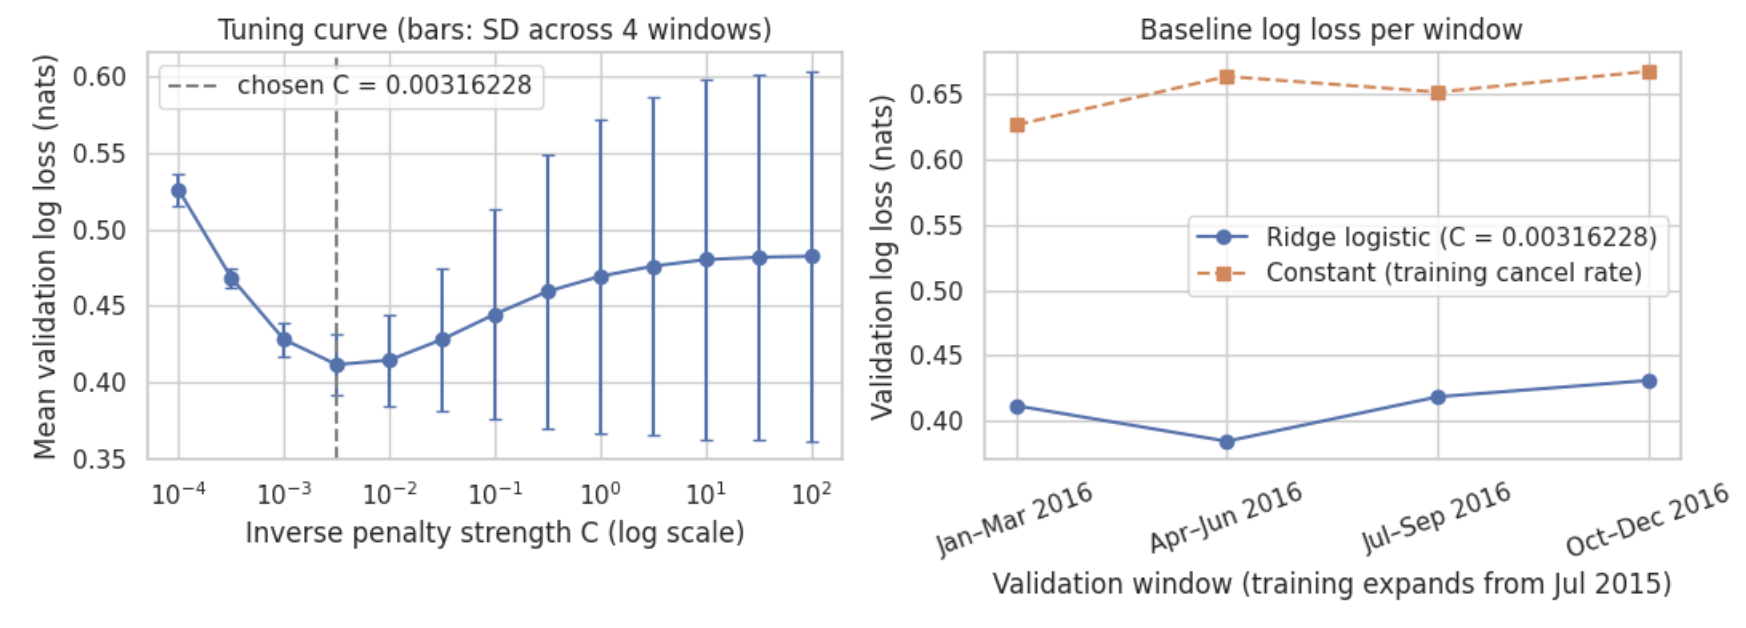
\includegraphics[width=0.85\linewidth]{baseline_performance.png}
    \caption{Ridge baseline validation performance. Left: mean log loss
    versus $C$ (error bars: SD across windows; dashed line: selected
    $C$). Right: log loss per window, with the constant forecast as a
    reference.}
    \label{fig:baseline-performance}
\end{figure}

\subsection{Tree-based comparators}

\textbf{Decision tree.}
The decision tree has a mean window log loss of 0.4990 and pooled
log loss of 0.4808. % TODO: state which fold / training set the 0.2573 refers to.
Its selected configuration has training log
loss of 0.2573, substantially lower than its mean validation loss,
consistent with a generalization gap. % TODO: name the feature(s) that define the 5,138-booking leaf, and explain what the 12.6--18.7% range refers to.
In the first validation
window, one leaf contains 5,138 bookings and accounts for 65.1\%
of that window's total log loss. The cancellation rate for this
group rises from approximately 0.2\% in the training period to
12.6\%--18.7\% in January--March 2016. The tree assigns this group
probabilities that are too low for the later period, illustrating
its sensitivity to a shift between the training and validation
periods, which may partly reflect seasonality because this training
set contains no earlier winter observations.

\textbf{Random forest.}
The random forest has a mean window log loss of 0.4127 and a pooled
log loss of 0.4067. Averaging across trees avoids the single-leaf
failure of the decision tree, but the forest is not uniformly better
than the baseline: its first-window loss of 0.4805 is worse than
ridge's 0.4118, even though it performs better than ridge in the
final three windows.

\subsection{Model comparison}

\textbf{Overall validation performance.}
Table~\ref{tab:validation-results} summarizes the three models'
out-of-window performance. Ridge logistic regression and the random
forest are close (mean window log loss 0.4116 and 0.4127), while the
decision tree performs worse at 0.4990. On average, all three models
improve substantially over the constant-probability reference, whose
mean window log loss is 0.6517. The exception is the decision tree in
the first window (0.7308), which is worse than the constant forecast
(0.6259).

\begin{table}[H]
    \caption{Preliminary out-of-window validation performance.
    Mean window log loss is the unweighted average across the four
    quarterly validation windows. Pooled log loss is calculated
    over all out-of-window predictions. Bracketed values give
    95\% weekly-block bootstrap intervals based on 2,000 resamples.
    Lower log loss is better; ROC-AUC is secondary. The constant
    forecast is a reference, not a model baseline. The 2017 test
    cohort is excluded.}
    \label{tab:validation-results}
    \centering
    \small
    \setlength{\tabcolsep}{4pt}
    \begin{tabular}{lccc}
        \toprule
        Model & Mean window log loss &
        Pooled log loss (95\% CI) & Mean AUC \\
        \midrule
        Ridge logistic (baseline) & 0.4116 & 0.4108 [0.3983, 0.4247] & 0.8811 \\
        Decision tree & 0.4990 & 0.4808 [0.4410, 0.5253] & 0.8571 \\
        Random forest & 0.4127 & 0.4067 [0.3880, 0.4264] & 0.8824 \\
        Constant forecast (reference) & 0.6517 & --- & --- \\
        \bottomrule
    \end{tabular}
\end{table}

\textbf{Performance across validation windows.}
Table~\ref{tab:window-results} reports each model's log loss in
the four validation periods. The decision tree has a particularly
high first-window loss of 0.7308, compared with 0.4118 for ridge
and 0.4805 for the random forest. Its performance is closer to
the other models in the remaining windows. The random forest
performs better than ridge in the final three windows but worse
in the first. This variation suggests that the relative performance
of the models changes across arrival cohorts. The first window also
has the smallest training set (21,967 bookings from July--December
2015, with no earlier winter observations), so its larger losses may
reflect seasonality or limited training data as well as temporal
change.

\begin{table}[H]
    \caption{Validation log loss by expanding-window period.
    Lower values are better. Values are rounded to four decimal
    places. The constant forecast is included as a reference.}
    \label{tab:window-results}
    \centering
    \small
    \begin{tabular}{lcccc}
        \toprule
        Validation window & Ridge logistic & Decision tree &
        Random forest & Constant forecast \\
        \midrule
        Jan--Mar 2016 & 0.4118 & 0.7308 & 0.4805 & 0.6259 \\
        Apr--Jun 2016 & 0.3847 & 0.3963 & 0.3554 & 0.6630 \\
        Jul--Sep 2016 & 0.4186 & 0.4297 & 0.4033 & 0.6510 \\
        Oct--Dec 2016 & 0.4311 & 0.4391 & 0.4118 & 0.6669 \\
        \midrule
        Mean & 0.4116 & 0.4990 & 0.4127 & 0.6517 \\
        \bottomrule
    \end{tabular}
\end{table}

\textbf{Paired comparisons.}
The paired pooled difference (random forest minus ridge) is
$-0.0041$ nats, with a 95\% interval of [$-0.0152$, $0.0081$].
Because this interval crosses zero, the results do not establish a
clear improvement over ridge. The decision-tree-minus-ridge
difference is $+0.0700$ [0.0347, 0.1099], favoring ridge. The
random-forest-minus-tree difference is $-0.0741$
[$-0.1027$, $-0.0477$], favoring the forest.
Figure~\ref{fig:model-comparison} presents the paired differences
across validation windows and the pooled bootstrap comparisons. The
forest performs better than the tree in all four windows, but its
advantage over ridge is not consistent across time.

\begin{figure}[H]
    \centering
    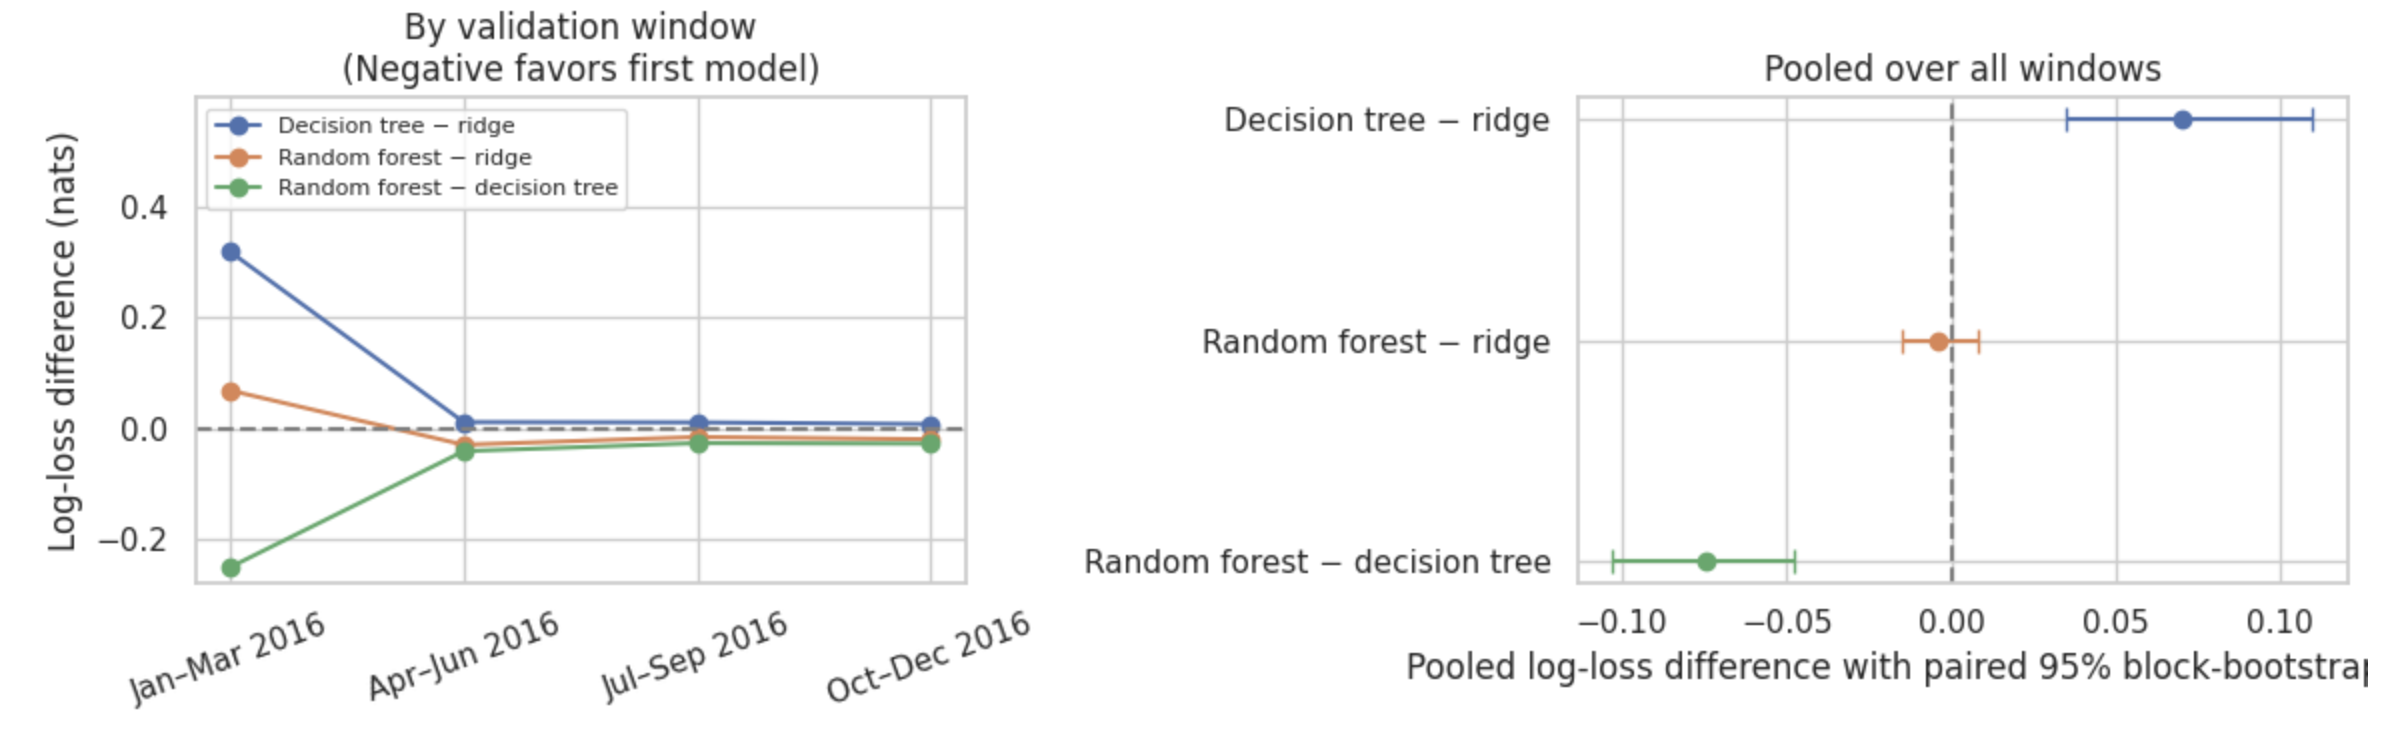
\includegraphics[width=\linewidth]{model_comparison.png}
    \caption{Pairwise model comparisons based on validation
    log loss. The left panel shows log-loss differences across
    the four validation windows. The right panel shows pooled
    log-loss differences with paired 95\% weekly-block bootstrap
    intervals based on 2,000 resamples. Negative values favor
    the first model in each comparison.}
    \label{fig:model-comparison}
\end{figure}

\section{Discussion and Limitations}

The preliminary results do not show that tree-based models
consistently improve cancellation prediction over ridge logistic
regression. The single decision tree has higher validation log
loss and is particularly sensitive to the first validation period.
The random forest is more competitive, but its average performance
is close to ridge and its paired bootstrap interval does not
establish a reliable improvement.

Several limitations remain. First, hyperparameters were selected
using the same four validation windows on which performance is
summarized, so the reported validation results may be optimistic.
The paired bootstrap quantifies uncertainty across weekly blocks
but does not correct this model-selection bias. Second, the data
are captured from booking change logs as of the day before arrival.
Some predictors may therefore contain information unavailable at
reservation creation. Third, apparent duplicate records remain in
the main analysis and require a sensitivity check.

The January--August 2017 cohort remains held out. Final conclusions
will be based on a one-time evaluation after the feature set,
preprocessing, and hyperparameters have been frozen.

\section{Remaining Work}

The remaining analyses are targeted for completion by Monday,
November 30:

\begin{enumerate}
    \item \textbf{Predictor-timing sensitivity.}
    Repeat the four validation windows after removing
    \texttt{deposit\_type}, then
    \texttt{required\_car\_parking\_spaces} and
    \texttt{total\_of\_special\_requests}, and finally all three
    fields together. Keep the main-analysis hyperparameters fixed
    to isolate feature dependence, and refit preprocessing within
    each training window.

    \item \textbf{Duplicate-record sensitivity.}
    Compare the main analysis with a version that removes exact
    duplicate rows. Examine whether duplicated observations across
    training and validation periods affect the results. Because
    flexible models can memorize repeated rows, this check may matter
    more for the tree and forest than for ridge, so it will be run
    before the protocol is frozen.

    \item \textbf{Freeze the modeling protocol.}
    Complete the feature-timing audit, confirm that all models use
    the same development rows and folds, document any changes,
    and freeze preprocessing, feature sets, and hyperparameters.

    \item \textbf{Held-out evaluation.}
    Refit each selected pipeline on all 78,590 development bookings
    and evaluate once on the 40,619 January--August 2017 bookings.
    Report test log loss, ROC-AUC, paired weekly-block bootstrap
    differences from ridge, and threshold diagnostics in an
    appendix. No tuning will be performed on the test cohort.

    \item \textbf{Complete the paper.}
    Add final test results, robustness checks, a discussion of
    temporal generalization and feature-timing limitations, model
    importance results, and appendix diagnostics.
\end{enumerate}

\begin{thebibliography}{9}

\bibitem[Antonio et al.(2019)]{antonio2019hotel}
Antonio, N., de Almeida, A., and Nunes, L.
\newblock Hotel booking demand datasets.
\newblock \textit{Data in Brief}, 22:41--49, 2019.
\newblock doi:10.1016/j.dib.2018.11.126.

\end{thebibliography}

\end{document}